\documentclass[14pt,mathserif,dvipsnames,usenames]{beamer}
\usepackage[noend]{algorithmic}
\usepackage{latexsym,amsmath,url}
\usepackage{hyperref}
\usepackage{color}
\DeclareSymbolFont{AMSb}{U}{msb}{m}{n}
\DeclareMathSymbol{\N}{\mathbin}{AMSb}{"4E}
 \DeclareMathOperator*{\argmax}{argmax}
 \DeclareMathOperator*{\argmin}{argmin}
 \DeclareMathOperator*{\sign}{sign}
\newcommand{\vecb}[1]{\mathbf{#1}}
\newcommand{\x}{\mathbf{x}} 
\newcommand{\y}{\mathbf{y}}
\newcommand{\w}{\mathbf{w}}
\newcommand{\W}{\mathbf{W}}

 \newcommand{\voc}[1]{{\color{ForestGreen}#1}}
%\newcommand{\voc}[1]{#1}

\newcommand{\superscript}[1]{\ensuremath{^\textrm{\scriptsize#1 }}}
\mode<presentation>{ 
  \usetheme{Boadilla}
} \title[Linear models ]{ Linear models for classification }


\author[Chrupala and Stroppa]{Grzegorz Chrupa{\l}a and Nicolas Stroppa}

\institute[UdS] % (optional, but mostly needed)
{
Saarland University\\
Google
}
\date[2010] % (optional, should be abbreviation of conference name)
{META Workshop}


%\pgfdeclareimage[height=1cm]{UdS}{SaarlandUniversityLogo.jpg}
%\logo{\pgfuseimage{UdS}}

 \AtBeginSection[]
 {
    \begin{frame}
        \frametitle{Outline}
        \tableofcontents[currentsection]
    \end{frame}
 }
\begin{document}
\frame{\titlepage}

\begin{frame}
  \frametitle{Outline}
  \tableofcontents
\end{frame}

\section{Linear models}

\begin{frame}
\frametitle{An example}
Positive examples are blank, negative are filled
\begin{center}
\vskip -0.5cm 
\includegraphics[scale=0.4]{linear.pdf}
\end{center}
\end{frame}

\begin{frame}
  \frametitle{Linear models}
  \begin{block}{}
    Think of \voc{training examples} as points in $d$-dimensional
    space. Each dimension corresponds to one \voc{feature}.
  \end{block}
  \begin{block}{}
    A linear binary classifier defines a plane in the space which
    separates \voc{positive} from \voc{negative} examples. 
  \end{block}
\end{frame}

\begin{frame}
 \frametitle{Linear decision boundary}
\begin{itemize}
\item A \voc{hyperplane} is a generalization of a straight line to
  $>2$ dimensions
\item A hyperplane contains all the points in a $d$ dimensional space satisfying the following equation:
\[
 w_1x_1 + w_2x_2, \ldots, + w_dx_d + w_0 = 0
\]
\item Each coefficient $w_i$ can be thought of as a weight on the
  corresponding feature
\item The vector containing all the weights $\w = (w_0,\ldots,w_d)$ is the
  \voc{parameter vector} or \voc{weigth vector}
\end{itemize}
\end{frame}



\begin{frame}
 \frametitle{Normal vector}
\begin{itemize}
\item Geometrically, the weight vector $\w$ is a \voc{normal vector}
  of the separating hyperplane
\item A normal vector of a surface is any vector which is
  perpendicular to it
\begin{center}
 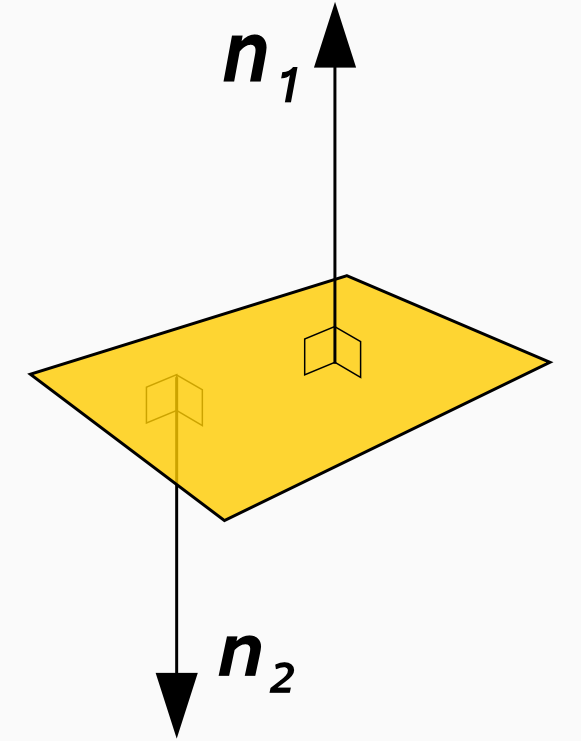
\includegraphics[scale=0.2]{Normal_vectors2.png}
 \end{center}
\end{itemize}
\end{frame}


 \begin{frame}\frametitle{Hyperplane as a classifier}
   \begin{itemize}
   \item Let \[
     g(\x) =  w_1x_1 + w_2x_2, \ldots, + w_dx_d + w_0
     \]
 \item Then
   \[ y = \sign( g(\x) ) =
   \begin{cases}
    +1 & \text{ if } g(\x) \geq 0\\
    -1 & \text{ otherwise }
   \end{cases}
 \]
   \end{itemize}
 \end{frame}

\begin{frame}
 \frametitle{Bias}
\begin{itemize}
\item The slope of the hyperplane is determined by
  $w_1...w_d$. The location (intercept) is determined by  bias $w_0$
\item Include bias in the
  weight vector and add a dummy component to the feature vector
\item Set this component to $x_0 = 1$
\item Then 
 \begin{align*}
 g(\x) & = \sum_{\alert{i=0}}^d w_i x_i\\
 g(\x) & = \w \cdot \x
\end{align*}
\end{itemize}
\end{frame}

\begin{frame}
\label{hyperplanes}
\frametitle{Separating hyperplanes in 2 dimensions}
\begin{center}
\vskip -0.5cm 
\includegraphics[scale=0.5]{linear.pdf}
\end{center}
\end{frame}

\begin{frame}
 \frametitle{Learning}
\begin{itemize}
\item The goal of the learning process is to come up with a ``good''
  weight vector $\w$
\item The learning process will use examples to guide the search of a
  ``good'' $\w$
\item Different notions of ``goodness'' exist, which yield different
  learning algorithms
\item We will describe some of these algorithms in the following
\end{itemize}
\end{frame}


\section{Perceptron}
\begin{frame}
 \frametitle{Perceptron training}
\begin{itemize}
 \item How do we find a set of weights that separate our classes?
\item \textbf{Perceptron}: A simple mistake-driven online algorithm
\begin{block}{}
\begin{itemize}
\item Start with a zero weight vector and process each training
  example in turn.
\item If the current weight vector classifies the current example
  incorrectly, move the weight vector in the right direction.
\item If weights stop changing, stop
\end{itemize}
\end{block}
\item If examples are linearly separable, then this algorithm is
  guaranteed to converge to the solution vector
\end{itemize}
\end{frame}

\begin{frame}
 \frametitle{Fixed increment online perceptron algorithm}
\begin{itemize}
\item Binary classification, with classes $+1$ and $-1$
\item Decision function $y' = \mathrm{sign}(\vecb{w}\cdot \x)$
\end{itemize}

\begin{block}{\textsc{Perceptron}($x^{1:N},y^{1:N},I$):}
\begin{algorithmic}[1]
\STATE $\vecb{w} \leftarrow \vecb{0}$
\FOR {$i = 1...I$}
	\FOR {$n = 1...N$}
    		\IF {$y^{(n)} (\vecb{w}\cdot \x^{(n)}) \leq 0$}
        		\STATE $\vecb{w} \leftarrow \vecb{w} + y^{(n)} \x^{(n)}$
    		\ENDIF
    	\ENDFOR
\ENDFOR
\STATE \textbf{return} $\vecb{w}$
\end{algorithmic}                 \end{block}
\end{frame}


\begin{frame}
  \frametitle{Or more explicitly}
\begin{algorithmic}[1]
\STATE $\vecb{w} \leftarrow \vecb{0}$
\FOR {$i = 1...I$}
  \FOR {$n = 1...N$}
    \IF {$y^{(n)} = \sign(\w\cdot \x^{(n)}) $}
      \STATE pass
      \ELSIF { $y^{(n)} = +1 \wedge \sign(\w\cdot\x^{(n)}) = -1$ }
      \STATE $\w \leftarrow \w + \x^{(n)}$
      \ELSIF { $y^{(n)} = -1 \wedge \sign(\w\cdot\x^{(n)}) = +1$ }
      \STATE $\w \leftarrow \w - \x^{(n)}$
    \ENDIF
   \ENDFOR
  \ENDFOR
\STATE \textbf{return} $\vecb{w}$
\end{algorithmic}
\end{frame}

\begin{frame}
 \frametitle{Weight averaging}
\begin{itemize}
\item Although the algorithm is guaranteed to converge, the solution
  is not unique!
\item Sensitive to the order in which examples are processed
\item Separating the training sample does not equal good accuracy on
  unseen data
\item Empirically, better generalization performance with
  \voc{weight averaging}
\begin{itemize}
\item A method of avoiding overfitting
\item As final weight vector, use the mean of all the weight vector
  values for each step of the algorithm
\item (cf.\ regularization in a following session)
\end{itemize}
\end{itemize}
\end{frame}


\section{Na{\"i}ve Bayes}
\begin{frame}
  \frametitle{Probabilistic model}
  \begin{itemize}
  \item Instead of thinking in terms of multidimensional space...
  \item Classification can be approached as a probability estimation problem
  \item We will try to find a probability distribution which
    \begin{itemize}
    \item  Describes
    well our training data 
  \item Allows us  to make accurate predictions 
    \end{itemize}
  \item We'll look at Naive Bayes as a simplest example of a
    probabilistic classifier
  \end{itemize}
\end{frame}


\begin{frame}
  \frametitle{Representation of examples}
  \begin{itemize}
    \item We are trying to classify documents. Let's
    represent a document as a sequence of terms (words) it contains
    $\mathbf{t} = (t_1...t_n)$

  \item For (binary) classification we want to find the most probable class:
    \[ \hat{y} = \argmax_{y \in \{-1,+1\}} P(Y=y|\mathbf{t}) \]
  \item But documents are close to unique: we cannot reliably
    condition $Y|\mathbf{t}$
  \item Bayes' rule to the rescue
  \end{itemize}
\end{frame}


\begin{frame}
  \frametitle{Bayes rule} Bayes rule determines how joint and
  conditional probabilities are related.
 
  \begin{block}{}
\[
P(Y=y_i|X=x) = \frac{P(X=x|Y) P(Y=y_i)}{\sum_i P(X=x|Y=y_i)
  P(Y=y_i)}
\]
That is:
\[
\mbox{posterior} = \frac{\mbox{prior} \times
  \mbox{likelihood}}{\mbox{evidence}}
\]
\end{block}
\end{frame}

\begin{frame}
  \frametitle{Prior and likelihood}
  \begin{itemize}
  \item With Bayes' rule we can invert the direction of conditioning
\begin{align}\nonumber
\hat{y} & = \argmax_y \frac{P(Y=y)P(\mathbf{t}|Y=y)}{\sum_y P(Y=y)P(\mathbf{t}|Y=y) }\\\nonumber
        & = \argmax_y P(Y=y)P(\mathbf{t}|Y=y)
\end{align}
\item Decomposed the task into estimating the prior $P(Y)$ (easy) and
  the likelihood $P(\mathbf{t}|Y=y)$
  \end{itemize}
\end{frame}


\begin{frame}
  \frametitle{Conditional independence}
  \begin{itemize}
  \item How to estimate $P(\mathbf{t}|Y=y)$?
  \item \alert{Naively} assume the occurrence of each word in the
    document is independent of the others, when conditioned on the
    class
    \[
    P(\mathbf{t}|Y=y) = \prod_{i=1}^{|\mathbf{t}|} P(t_i|Y=y)
    \]
  \end{itemize}
\end{frame}



\begin{frame}\frametitle{Naive Bayes}
  \begin{block}{Putting it all together}
    \[
   \hat{y} = \argmax_y P(Y=y)\prod_{i=1}^{|\mathbf{t}|} P(t_i|Y=y)
    \]
\end{block}
\end{frame}


\begin{frame}\frametitle{Decision function}
\begin{itemize}
  \item For binary classification:
    \begin{align}\nonumber
    g(\mathbf{t}) & = \frac{P(Y=+1)\prod_{i=1}^{|\mathbf{t}|} P(t_i|Y=+1)}
                {P(Y=-1)\prod_{i=1}^{|\mathbf{t}|} P(t_i|Y=-1)}\\\nonumber
         & = \frac{P(Y=+1)}{P(Y=-1)}\prod_{i=1}^{|\mathbf{t}|} \frac{P(t_i|Y=+1)}{P(t_i|Y=-1)}
    \end{align}
    \[
    \hat{y} = 
    \begin{cases}
      +1 \text{ if } g(\mathbf{t}) \geq 1\\
      -1 \text{ otherwise }
    \end{cases}
    \]
  \end{itemize}
\end{frame}

\begin{frame}
  \frametitle{Documents in vector notation}
  \begin{itemize}
  \item Let's represent documents as vocabulary-size-dimensional
    binary vectors 

    \begin{tabular}{rlllll}
          &    $V_1$& $V_2$   & $V_3$   & $V_4$   & \\\hline
          & Obama   & Ferrari & voters  & movies & \\\hline
$\x = ($   & 1       & 0       & 2       & 0 & $)$\\
    \end{tabular}
  \item Dimension $i$ indicates how many times the $i^{th}$ vocabulary
    item appears in document $\x$
  \end{itemize}
\end{frame}

\begin{frame}
  \frametitle{Naive Bayes in vector notation}
  \begin{itemize}
  \item 
    Counts appear as exponents:
    \[
      g(\x) = \frac{P(+1)}{P(-1)} \prod_{i=1}^{|V|} \left(\frac{P(V_i|+1)}{P(V_i|-1)}\right)^{\color{blue} x_i}
    \]
  \item If we take the logarithm of the threshold ($\ln 1 = 0$) and
    $g$, we'll get the same decision function
    \begin{align*}
      h(\x) = \ln\left(\frac{P(+1)}{P(-1)}\right) + \sum_{i=1}^{|V|} \ln\left(\frac{P(V_i|+1)}{P(V_i|-1)}\right)\color{blue}x_i
    \end{align*}
  \end{itemize}
\end{frame}

\begin{frame}
  \frametitle{Linear classifier}
  \begin{itemize}
  \item Remember the linear classifier?
    \begin{align}\nonumber
      g(\x) = & w_0               &  & + \sum_{i=1}^d      && w_i 
                            & x_i \\\nonumber
      h(\x) = &  \ln\left(\frac{P(+1)}{P(-1)}\right)      &  & + \sum_{i=1}^{|V|}  &&  \ln\left(\frac{P(V_i|+1)}{P(V_i|-1)}\right)
                            & x_i 
    \end{align} 
  \item Log prior ratio corresponds to the bias term
  \item Log likelihood ratios correspond to feature weights
  \end{itemize}
\end{frame}


\begin{frame}
  \frametitle{What is the difference}
  Training criterion and procedure
  \begin{block}{Perceptron}
    \begin{itemize}
    \item Zero-one loss function    
      \[
      \mathit{error}(\w,D) = \sum_{(\x,y) \in D}
      \begin{cases}
        0 \text{ if } \sign(\w \cdot \x) = y\\
        1 \text{ otherwise }
      \end{cases}
      \]
    \item Error-driven algorithm
    \end{itemize}
  \end{block}
\end{frame}

\begin{frame}
  \begin{block}{ Naive Bayes}
    \begin{itemize}
  \item Maximum Likelihood criterion 
    \[
    P(D|\theta) = \prod_{(\x,y) \in D} P(Y=y|\theta)P(x|Y=y,\theta)
    \]
  \item Find parameters which maximize the log likelihood
    \begin{align}\nonumber
    \hat{\theta} & = \argmax_{\theta} \log(P(D|\theta))
    \end{align}
    Parameters reduce to relative counts
  \item + Ad-hoc smoothing
  \item Alternatives (e.g.\ maximum {\it a posteriori})
  \end{itemize}
\end{block}
\end{frame}

\begin{frame}
  \frametitle{Comparison}
  \begin{center}
  \begin{tabular}{l|l|l}
    Model          & Naive Bayes & Perceptron \\\hline
    Model power    & Linear      & Linear\\
    Type           & Generative  & Discriminative\\
    Distribution 
    modeled        & $P(\x,y)$   & N/A \\
    Smoothing      & Crucial     & Optional\\
    Independence 
    assumptions    & Strong      & None \\
  \end{tabular}   
  \end{center}
\end{frame}


\section{Logistic regression}

\begin{frame}\frametitle{Probabilistic \voc{conditional} model}
  \begin{itemize}
  \item Let's try to come up with a \voc{probabilistic model} which
    has some of the advantages of perceptron
  \item Model $P(y|\x)$ directly, and not via $P(\x,y)$ and Bayes rule
    as in Naive Bayes
  \item Avoid issue of dependencies between features of $\x$
  \item We'll take \voc{linear regression} as a starting point
    \begin{itemize}
    \item The goal is to adapt regression to model class-conditional
      probability 
    \end{itemize}
  \end{itemize}
\end{frame}

\begin{frame}
\frametitle{Linear Regression}
 \begin{itemize}
 \item Training data: observations paired with outcomes ($n \in
   \mathbb{R}$)
 \item Observations have features (predictors, typically also real
   numbers)
 \item The model is a \voc{regression line} $y = ax + b$ which best
   fits the observations
   \begin{itemize}
   \item $a$ is the \voc{slope}
   \item $b$ is the \voc{intercept}
   \item This model has two parameters (or weigths)
   \item One feature = $x$ 
   \item Example: \begin{itemize}
     \item $x$ = number of vague adjectives in property
       descriptions
     \item $y$ = amount house sold over asking price
     \end{itemize}
   \end{itemize}
 \end{itemize}
\end{frame}

\begin{frame}
\begin{center}
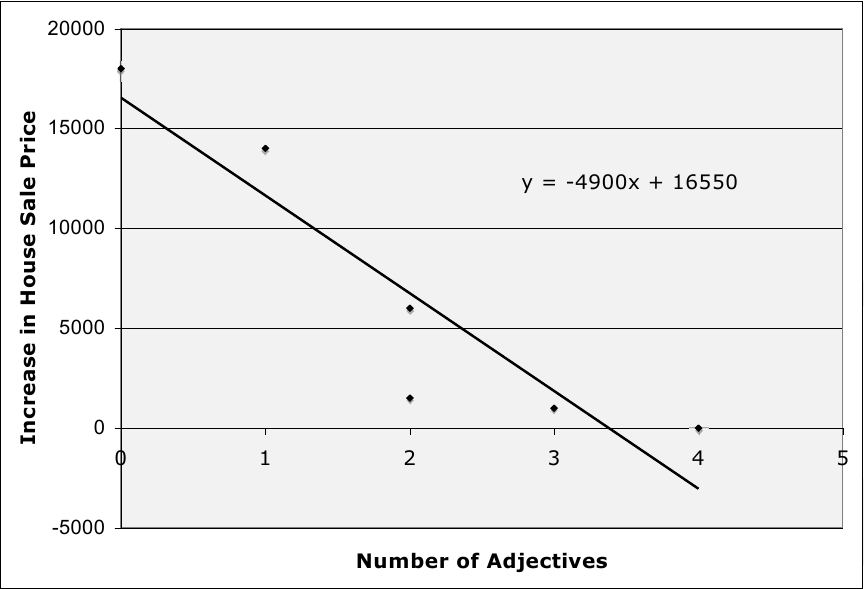
\includegraphics[scale=0.3]{regressionjm.png}
% regressionjm.png: 864x589 pixel, 72dpi, 30.48x20.78 cm, bb=0 0 864 589

\end{center}
\end{frame}


\begin{frame}
\frametitle{Multiple linear regression}
\begin{itemize}
\item More generally $y = w_0 + \sum_{i=1}^{d} w_i x_i$, where
  \begin{itemize}
  \item $y$ = outcome
  \item $w_0$ = intercept
  \item $x_1..x_d$ = features vector and $w_1 .. w_d$ weight vector
    \item Get rid of bias:
      \[
      g(\x) = \sum_{i=0}^d w_i x_i = \w \cdot \x 
      \]
 \end{itemize}
 
  \item Linear regression: uses $g(\x)$ directly
  \item Linear classifier: uses $\sign(g(\x))$
\end{itemize}
\end{frame}

\begin{frame}
  \frametitle{Learning linear regression}
  \begin{itemize}
  \item Minimize \voc{sum squared error} over $N$ training examples 
    \[ \mathrm{Err}(\w) = \sum_{n=1}^{N}(g(\x^{(n)}) - y^{(n)})^2 \]
  \item Closed-form formula for choosing the best weights $\w$:
    \[ \w = (X^{T}X)^{-1} X^{T} \mathbf{y} \] where the matrix $X$
    contains training example features, and $\mathbf{y}$ is the vector
    of outcomes.
\end{itemize}
\end{frame}

\begin{frame}
\frametitle{Logistic regression}
\begin{itemize}
\item In logistic regression we use the linear model to assign
  probabilities to class labels
\item For binary classification, predict $P(Y=1|\x)$. But predictions
  of linear regression model are $\in \mathbb{R}$, whereas
  $P(Y=1|\x) \in [0,1]$
\item Instead predict logit function of the probability:
\begin{align*}
  \ln\left(\frac{ P(Y=1|\x) }{1-P(Y=1|\x)}\right) & = \w\cdot\x \\
  \frac{P(Y=1|\x)}{1-P(Y=1|\x)} & = e^{\w\cdot\x}
\end{align*}
\end{itemize}
\end{frame}


\begin{frame}
Solving for $P(Y=1|\x)$ we obtain:
\begin{align*}
  P(Y=1|\x)  & = e^{\w\cdot\x}(1-P(Y=1|\x))\\
  P(Y=1|\x)  & =  e^{\w\cdot\x} -  e^{\w\cdot\x}P(Y=1|\x)\\
  P(Y=1|\x) + e^{\w\cdot\x}P(Y=1|\x) & = e^{\w\cdot\x}\\
  P(Y=1|\x)(1  + e^{\w\cdot\x})      & = e^{\w\cdot\x}\\
  P(Y=1|\x) & = \frac{e^{\w\cdot\x}}{1+e^{\w\cdot\x}} \\
  & = \frac{\exp\left(\sum_{i=0}^d w_i
      x_i\right)}{1+\exp\left(\sum_{i=0}^d w_i x_i\right)}
\end{align*}
\end{frame}


\begin{frame}
 \frametitle{Logistic regression - classification}
\begin{itemize}
 \item Example $\x$ belongs to class $1$ if:
\begin{align*}
 \frac{P(Y=1|\x)}{1-P(Y=1|\x)} & > 1 \\
 e^{\w\cdot\x}   & > 1 \\
 \w\cdot\x       & > 0 \\
 \sum_{i=0}^{d} w_i x_i          & > 0 
\end{align*}
\item Equation $\w \cdot \x = 0$ defines a hyperplane with points above
  belonging to class $1$
\end{itemize}

\end{frame}


\begin{frame}
  \frametitle{Multinomial logistic regression}
  \begin{block}{}
    Logistic regression generalized to more than two classes
    \[
    P(Y=y|\x,\W)  = \frac{ \exp(\W_{y\bullet} \cdot \x) }
    {\sum_{y'}      \exp(\W_{y'\bullet} \cdot \x) }
    \]
  \end{block}
\end{frame}

\begin{frame}
  \frametitle{Learning parameters}
  \begin{itemize}
  \item Conditional likelihood estimation: choose the weights which
    make the probability of the observed values $y$ be the highest,
    given the observations $\x_i$
  \item For the training set with $N$ examples:
    \begin{align*}
      \mathbf{\hat{\W}} & = \argmax_{\W} \prod_{i=1}^{N}P(Y=y^{(n)}|\x^{(n)},\W)\\
      & = \argmax_{\W} \sum_{i=1}^N \log P(Y=y^{(n)}|\x^{(n)},\W)
    \end{align*}
  \end{itemize}
\end{frame}



  \begin{frame}
  \frametitle{Error function}
Equivalently, we seek the value of the parameters which
\alert{minimize} the error function:
  \begin{align*}
    \mathrm{Err}(\W,D) & = - \sum_{n=1}^N \log P(Y=y^{(n)}|\x^{(n)},\W)
  \end{align*}
where $D = \{(x^{(n)},y^{(n)})\}_{n=1}^N$
\end{frame}

\begin{frame}  \frametitle{A problem in convex optimization}
\begin{itemize}
\item L-BFGS (Limited-memory Broyden-Fletcher-Goldfarb-Shanno method)
\item gradient descent
\item conjugate gradient
\item iterative scaling algorithms
\end{itemize}
\end{frame}

\begin{frame}
  \frametitle{Stochastic gradient descent}
  \begin{block}{Gradient descent}
    \begin{itemize}
    \item A gradient is a slope of a function
    \item That is, a set of partial derivatives, one for each
      dimension (parameter)
    \item By following the gradient of a convex function we can
     \alert{descend} to the bottom (minimum) 
    \end{itemize}
  \end{block}
\end{frame}

\begin{frame}
  \begin{center}
    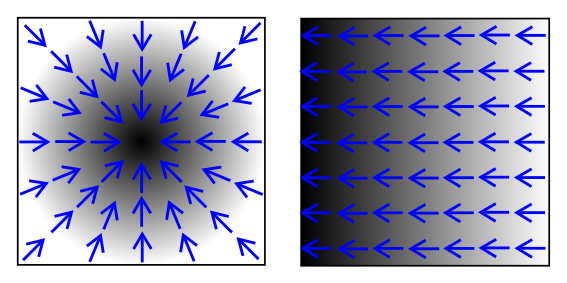
\includegraphics[scale=0.5]{Gradient2.png}
  \end{center}
\end{frame}

\begin{frame}\frametitle{Gradient descent example}
  \begin{itemize}
  \item Find $\argmin_{\theta} f(\theta)$ where $f(\theta) = \theta^2$
  \item Initial value of $\theta_1 = -1$
  \item Gradient function: $\nabla f(\theta) = 2 \theta$
  \item Update: $\theta^{(n+1)} = \theta^{(n)} - \eta \nabla f(\theta^{(n)})$
  \item The \voc{learning rate} $\eta$ ($=0.2$) controls the speed of
    the descent
    \pause
  \item After first iteration: $\theta^{(2)} = -1 - 0.2 (-2) = -0.6$
  \end{itemize}
\end{frame}

\begin{frame}\frametitle{Five iterations of gradient descent}
  \begin{center}
    \includegraphics[scale=0.5]{gradient.pdf}
  \end{center}
\end{frame}

\begin{frame}\frametitle{Stochastic}
  \begin{itemize}
  \item We could compute the gradient of error for the full dataset
    before each update
  \item Instead
    \begin{itemize}
    \item Compute the gradient of the error for a single example
    \item update the weight
    \item Move on to the next example
    \end{itemize}
  \item On average, we'll move in the right direction
  \item Efficient, \voc{online} algorithm
  \end{itemize}
\end{frame}


\begin{frame}
  \frametitle{Error gradient}
  \begin{itemize}
  \item The gradient of the error function is the set of
    partial derivatives of the error function with respect to the
    parameters $\W_{yi}$
    \begin{small}
      \begin{align*}
        \nabla_{y,i} \mathrm{Err}(D,\W) & = \frac{\partial}{\partial
          \W_{yi}} \left(- \sum_{n=1}^N \log
          P(Y=y|\x^{(n)},\W)\right)\\
        & = - \sum_{n=1}^N \frac{\partial}{\partial \W_{yi}} \log
        P(Y=y|\x^{(n)},\W)
      \end{align*}
    \end{small}
  \end{itemize}
\end{frame}

\begin{frame}
  \frametitle{Single training example}
  \begin{small}
    \begin{align*}
\frac{\partial}{\partial \W_{yi}} \log
        P(Y=y|\x^{(n)},\W)
      & = \frac{\partial }{\partial \W_{yi}} \log P(Y=y|\x^{(n)},\W) \\
      & = \frac{\partial }{\partial \W_{yi}} \log
      \frac{\exp(\W_{y\bullet} \cdot \x^{(n)})} {\sum_{y'}
        \exp(\W_{y'\bullet}
        \cdot \x^{(n)})}\\
      &  \cdots \\
      &  \cdots \\
      & = x_i^{(n)}(\mathbf{1}(y = y^{(n)})-P(Y=y|\x^{(n)},\W))
    \end{align*}
  \end{small}

\end{frame}

\begin{frame}\frametitle{Update}
\begin{block}{Stochastic gradient update step}
  \begin{small}
    \begin{align*}
      \W_{yi}^{(n)} & = \W_{yi}^{(n-1)} + \eta x_i^{(n)}(\mathbf{1}(y
      = y^{(n)})-P(Y=y|\x^{(n)},\W))
    \end{align*}
  \end{small}
  \end{block}
\end{frame}
  
\begin{frame}\frametitle{Update: Explicit}
  \begin{itemize}
  \item For the correct class ($y = y^{(n)}$)
    \[
    \W_{yi}^{(n)}  = \W_{yi}^{(n-1)} + \eta x_i^{(n)}(1-P(Y=y|\x^{(n)},\W))
    \]
    where $1-P(Y=y|\x^{(n)},\W)$ is the \voc{residual}\vskip 0.5cm
  \item For all other classes ($y \neq y^{(n)}$)
    \[
    \W_{yi}^{(n)}  = \W_{yi}^{(n-1)} - \eta x_i^{(n)}P(Y=y|\x^{(n)},\W)
    \]
  \end{itemize}
\end{frame}

\begin{frame}
  \frametitle{Logistics Regression SGD vs Perceptron}
\begin{align*}
\w^{(n)}  & = & \w^{(n-1)} + && 1 & \x^{(n)} & \\
    \W_{yi}^{(n)}  & = & \W_{yi}^{(n-1)} + && \eta & x_i^{(n)}& (1-P(Y=y|\x^{(n)},\W))
  \end{align*}
  \begin{itemize}
  \item Very similar update!
  \item Perceptron is simply an instantiation
    of SGD for a particular error function
  \item The perceptron criterion: for a correctly
    classified example zero error; for a misclassified example
    $-y^{(n)}\w\cdot\x^{(n)}$
  \end{itemize}
\end{frame}

\begin{frame}
  \frametitle{Maximum entropy}
  \begin{block}
    {}
Multinomial logistic regression model is also known as the \voc{Maximum entropy
model}. What is the connection?
  \end{block}
\end{frame}

\begin{frame}\frametitle{Entia non sunt multiplicanda praeter necessitatem}
 \begin{center}
 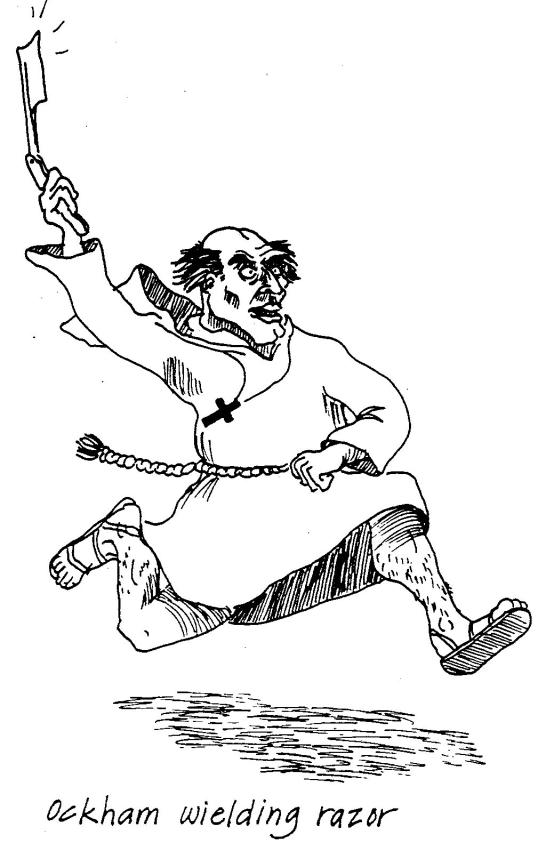
\includegraphics[]{ockham_razor.jpg}
 % ockham_razor.jpg: 546x851 pixel, 300dpi, 4.62x7.21 cm, bb=0 0 131 204
\end{center}
\end{frame}


\begin{frame}\frametitle{Maximum Entropy principle}
 \begin{block}{Jaynes, 1957}
   \begin{small}
     ... in making inferences on the basis of partial information we
     must use that probability distribution which has \alert{maximum
       entropy} subject to whatever is known. This is the only
     \alert{unbiased} assignment we can make; to use any other would amount to
     arbitrary assumption of information which we by hypothesis do not
     have.
   \end{small}
 \end{block}
\end{frame}


\begin{frame}
 \frametitle{Entropy}
\begin{itemize}
\item Out of all possible models, choose the simplest one consistent
  with the data
 \item Entropy of the distribution of $X$:
\[ H(X) = -\sum_{x}P(X=x)\log_2P(X=x) \] 
\item The uniform distribution has the \alert{highest entropy}
\end{itemize}
\end{frame}

\begin{frame}
\begin{itemize}
\item Finding the maximum entropy distribution:
\[
 p* = \argmax_{p\in C} H(p)
\]
\item Berger et al. (1996) showed that solving this problem is
  equivalent to finding the multinomial logistic regression model
  whose weights maximize the likelihood of the training data.
\end{itemize}
\end{frame}


\begin{frame}
 \frametitle{Maxent principle -- simple example}
\begin{itemize}
\item Find a Maximum Entropy probability distribution $p(a,b)$ where
  $a \in \{x,y\}$ and $b \in \{0,1\}$
\item The only thing we know are is the following constraint: 
  $p(x,0) + p(y,0) = 0.6$
 \end{itemize}
 \begin{center}
   
\begin{tabular}{l|ll|l}
 $p(a,b)$ & 0 & 1 & \\\hline
$x$       & ? & ? & \\
$y$       & ? & ? & \\\hline 
total     & 0.6 & & 1
\end{tabular}
\end{center}
\pause 
\begin{center}

\begin{tabular}{l|ll|l}
 $p(a,b)$ & 0 & 1 & \\\hline
$x$       & 0.3 & 0.2 & \\
$y$       & 0.3 & 0.2 & \\\hline
total     & 0.6 & & 1
\end{tabular}
\end{center}
\end{frame}


\begin{frame}
  \frametitle{Comparison}
  \begin{center}
    \begin{small}
      \begin{tabular}{l||l|l|l}
        Model          & Naive Bayes & Perceptron     & Log. regression \\\hline
        Model power    & Linear      & Linear         & Linear         \\
        Type           & Generative  & Discriminative & Discriminative \\
        Distribution   & $P(\x,y)$   & N/A            & $P(y|\x)$         \\
        Smoothing      & Crucial     & Optional$^1$   &
        Optional\footnote{Aka regularization} \\
        Independence & Strong      & None           & None\\
      \end{tabular}
    \end{small}
  \end{center}
\end{frame}


\begin{frame}
  \frametitle{The end}
\end{frame}

\begin{frame}
\frametitle{Efficient averaged perceptron algorithm}
 \begin{block}{\textsc{Perceptron}($x^{1:N},y^{1:N},I$):}
\begin{algorithmic}[1]
\STATE $\vecb{w} \leftarrow \vecb{0}$ ; $\vecb{w_a} \leftarrow \vecb{0}$
\STATE $b \leftarrow 0$ ; $b_a \leftarrow 0$
\STATE $c \leftarrow 1$
\FOR {$i = 1...I$}
	\FOR {$n = 1...N$}
    		\IF {$y^{(n)} (\vecb{w}\cdot \x^{(n)}+b) \leq 0$}
        		\STATE $\vecb{w} \leftarrow \vecb{w} + y^{(n)} \x^{(n)}$ ; $b \leftarrow b + y^{(n)}$
			\STATE $\vecb{w_a} \leftarrow \vecb{w_a} + c y^{(n)} \x^{(n)}$ ; $b_a \leftarrow b_a + c y^{(n)}$

    		\ENDIF
        \STATE $c \leftarrow c + 1$
    	\ENDFOR
\ENDFOR
\STATE \textbf{return} $(\vecb{w}-\vecb{w_a}/c, b - b_a/c)$
\end{algorithmic}                 \end{block}
\end{frame}


\end{document}


